% intro

Real-time Transport Protocol (RTP)~\cite{rfc3550} is suitable for multimedia
telephony (voice-over-IP, video conferencing, telepresence systems),
multimedia streaming (video-on-demand, live streaming), and multimedia
broadcast. RTP's design is based on the fundamental principles of \textit
{application-layer framing} and \textit{integrated layer
processing}~\cite{clark:alf}, i.e., it provides the following mechanisms:
source and payload type identification, packet playout time, stream
synchronization, packet loss and re-ordering, media stream monitoring.

Figure~\ref{fig:3:rtp.hdr} describes the RTP packet header format, the
\textit{`synchronisation source'} (SSRC) assists in determining the source
endpoint, typically useful when an endpoint sends multiple media streams that
need to be synchronized (e.g., Audio/Video lip-sync). The \textit{`RTP
timestamp'} assists in playing out the received packets at the appropriate
instance of time and recomposing the media frame from RTP packets. The
\textit{`RTP sequence number'} assists in identifying the lost packets and re-
ordering packets in case of out-of-order packet arrival. Lastly, RTP uses
\textit{`payload type'} (PT) to describe the encoding of the media data it is
carrying. Consequentely, each codec needs to specify its corresponding payload
format.

\begin{figure}[!htbp]
\centerline{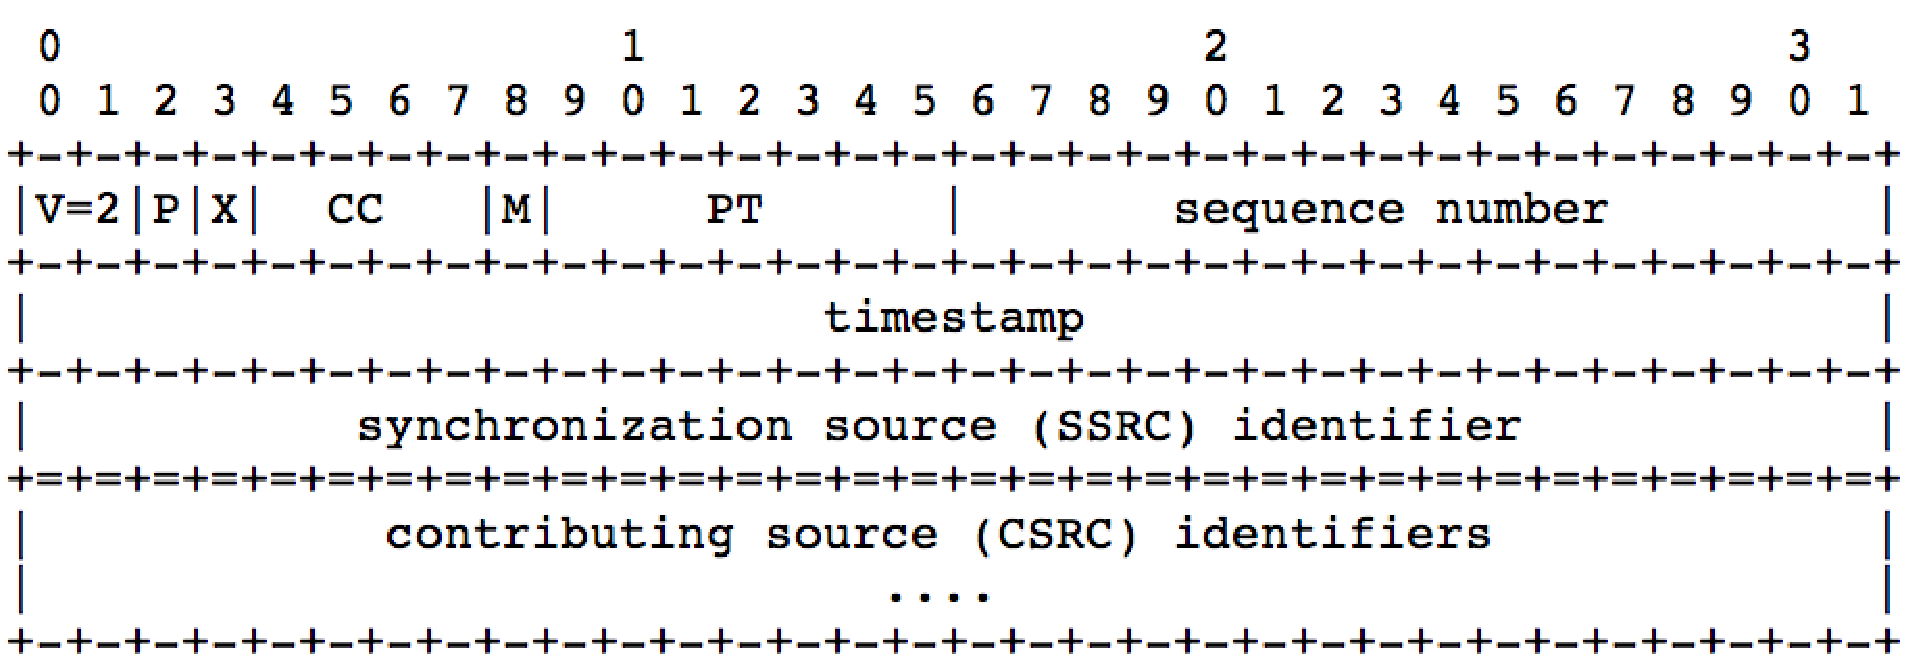
\includegraphics[width=\columnwidth]{fig_hdr_rtp}}
\caption{RTP header}
\label{fig:3:rtp.hdr}
\end{figure}

RTP utilizes RTP Control Protocol (RTCP) to monitor the performance of the
media stream. Using RTCP reports (RRs), the endpoints report loss fraction,
jitter, highest sequence number received, and calculate RTT. The RTCP reports
(SRs) also assist in synchronizing the media streams (audio and video) by
relating the RTP timestamps of the individual media streams to the wall clock
time and measuring RTT. Figure~\ref{fig:3:rtcp.hdr} describes the RTCP packet
header format for a unicast media stream.

\begin{figure}
\centerline{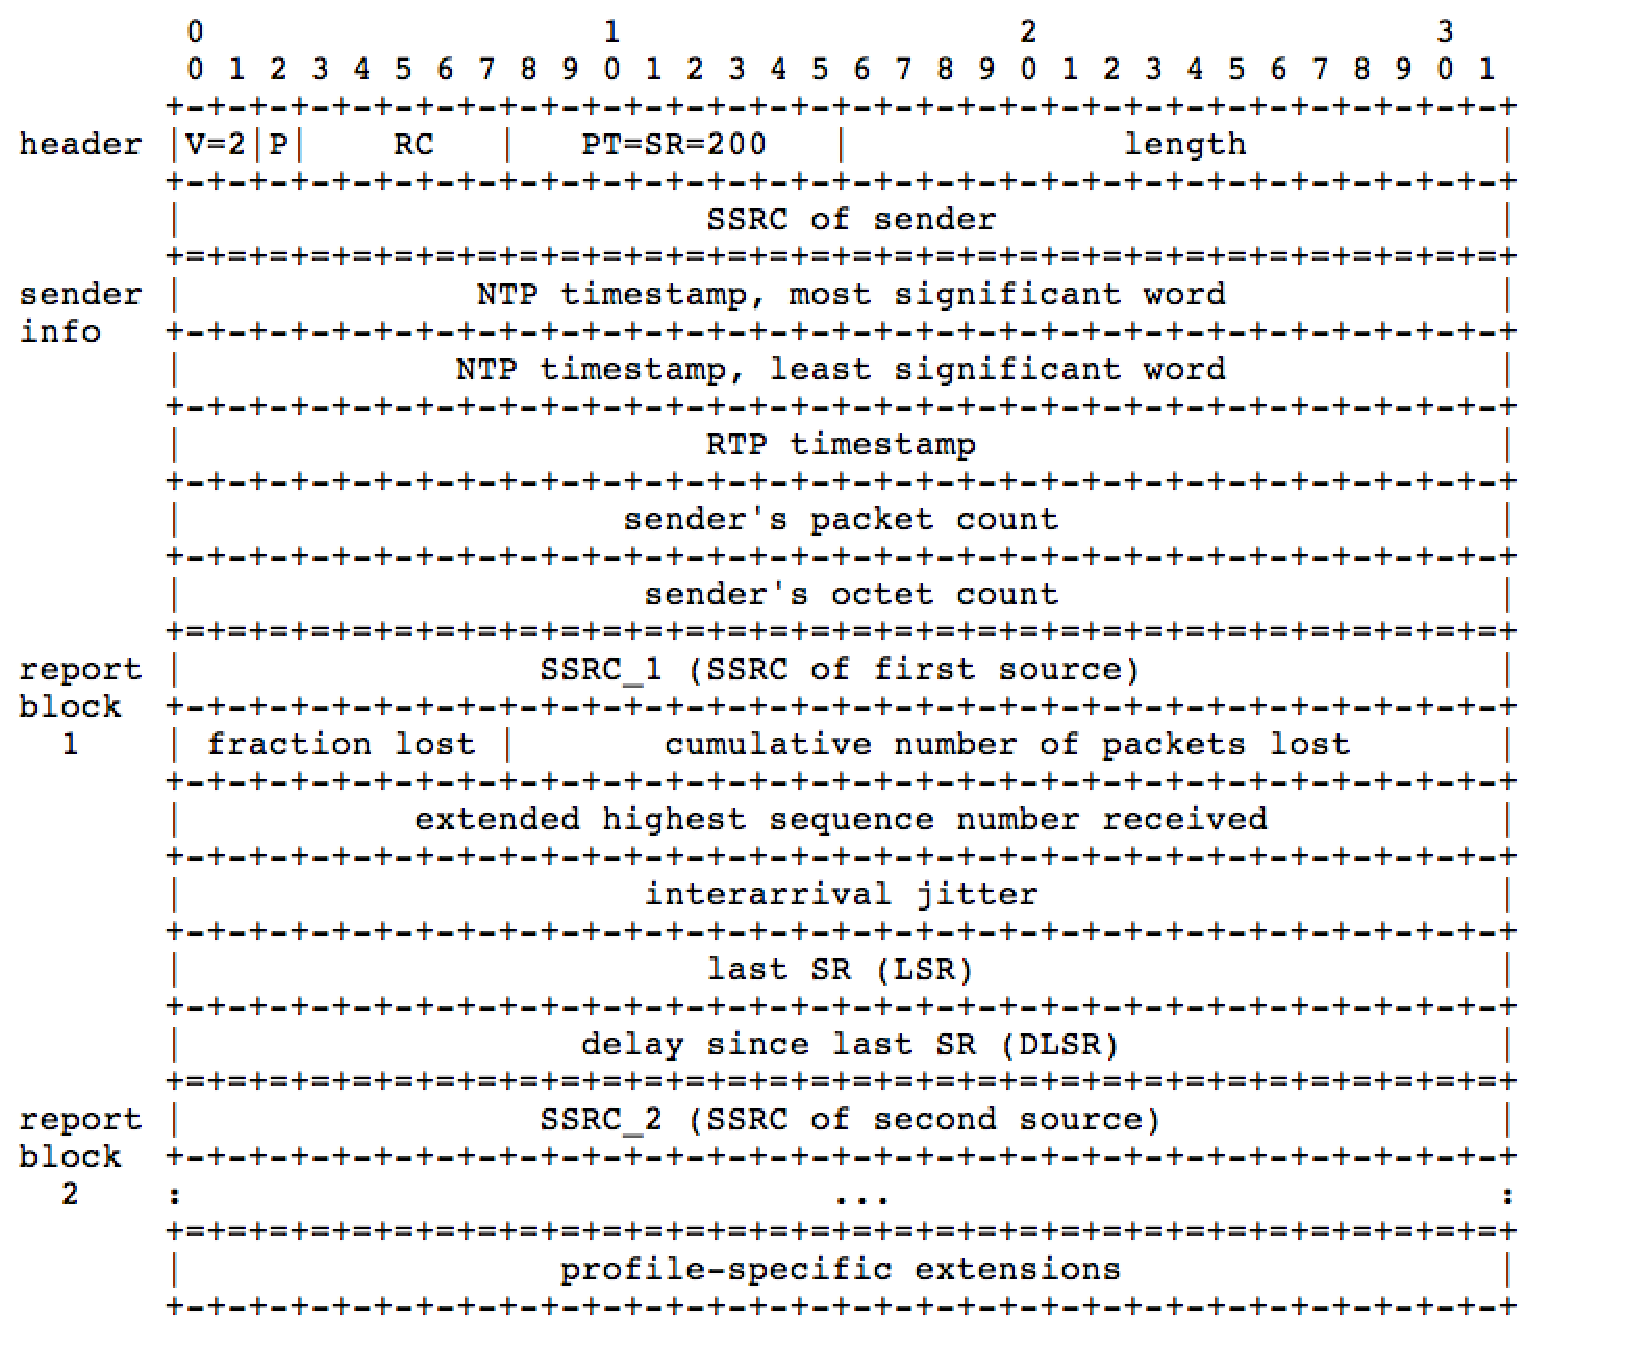
\includegraphics[width=\columnwidth]{fig_hdr_rtcp}}
\caption{RTCP header}
\label{fig:3:rtcp.hdr}
\end{figure}

\section{RTCP Reporting Interval}
% timing

A closed control loop is formed by sending RTP media packets and receiving
RTCP feedback packets. The RTCP reporting interval is determined by the number
of SSRCs in the session, and the chosen session bandwidth. Typically, in a
unicast session there are two SSRCs, one for each participant, but the number
of SSRCs can be higher if they send multiple media streams. The interval
between reports tends to be on the order of a few seconds, and is randomized
to avoid snchronization of reports from multiple endpoints. Formally, to
ensure that the RTCP reports are not sent too frequently, the endpoints limit
the feedback rate to $5\%$ of the session \textit{media rate}, half for each
participant. However, if the endpoint detects packet loss or onset of
congestion midway through a reporting interval, the base RTP
specification~\cite{rfc3550} (AVP profile) does not allow sending the RTCP
report early and the endpoint has to wait for the next scheduled RTCP report.
Hence, the slow control loop can cause instability and oscillation in the
media bit rate.

% avpf

Endpoints implement the Extended RTP Profile for RTCP-Based Feedback (AVPF
profile)~\cite{rfc4585}, an extension to RTP's default timing rules to enable
rapid feedback. This profile allows the endpoint to adjust the RTCP reporting
interval to send the RTCP feedback reports earlier than the next scheduled
RTCP report, sometimes even immidiately. As long as reporting interval on
average remains the same. Figure~\ref{fig:3:avpf.interval} shows the dynamics
of the AVPF-enabled RTCP reporting interval.

Along with the timely feedback, the AVPF profile also defines a suite of
error-resilience feedback messages, namely, Negative Acknowledgements (NACK),
Picture Loss Indication (PLI), Slice Loss Indication (SLI), Reference Picture
Selection Indication (RPSI).

\section{RTCP Extended Reports (XRs)}

Endpoints use RTCP XRs~\cite{rfc3611} to describe complex metrics that are not
exposed by the RTCP Receiver Report (RR). Some examples of XRs relevant to
performance monitoring and congestion control are: jitter buffer
metrics~\cite{draft.xr.jb}, Packet Delay Variation (PDV)~\cite{rfc6798}, summary
statistics~\cite{draft.xr.stat}, delay metric~\cite{rfc6843}, burst-gap
discard/loss~\cite{draft.xr.bg.loss, draft.xr.bg.discard}, Run-Length Encoded
(RLE) loss/discard~\cite{draft.xr.discard.rle}, Quality of Experience
(QoE)~\cite{draft.xr.qoe}, loss concealment~\cite{draft.xr.conceal}, etc.


% Transport Metrics

% The RTCP Extended Reports (XR) [RFC3611] allow reporting of more
% complex and sophisticated reception quality metrics, but do not
% change the RTCP timing rules.  RTCP extended reports of potential
% interest for congestion control purposes are the extended packet
% loss, discard, and burst metrics [RFC3611],
% [I-D.ietf-xrblock-rtcp-xr-discard],
% [I-D.ietf-xrblock-rtcp-xr-discard-rle-metrics],
% [I-D.ietf-xrblock-rtcp-xr-burst-gap-discard],
% [I-D.ietf-xrblock-rtcp-xr-burst-gap-loss]; and the extended delay
% metrics [RFC6843], [RFC6798].


\section{Codec Control}
% codec control

% relationship with SDP
\section{RTP Extensions}
\label{rtp.ext}
